% Chapter 1

\chapter{Introduction and Background} % Main chapter title

\label{Chapter1} % For referencing the chapter elsewhere, use \ref{Chapter1} 

\lhead{Chapter 1. \emph{Introduction and Background}} 
% This is for the header on each page - perhaps a shortened title

Nuclear reactors are extremely complicated systems, and modeling their 
dynamic behavior requires the solution of the neutron transport equation, a 
seven-dimensional ($\vec{r}$, $\vec{v}$, t) equation that describes the 
population of neutrons in the system.  Unfortunately, to solve the 
complete neutron transport equation is all but impossible for realistic 
problems 
without first reducing the problem space in some way.  For much of reactor 
analysis, it is reasonable to assume steady-state conditions, thus eliminating 
all time dependence from 
the problem.  In addition, it is very difficult to account for the energy 
dependence directly, and a common approach is to use the multigroup method, 
in which the energy variable is discretized into $G$ energy bins or 
``groups''.  After these assumptions and the further assumption of 
isotropic scattering, the 
neutron transport equation reduces to
\begin{equation}
    \begin{split}
    \vec{\hat{\Omega}}\cdot \nabla \psi_g(\vec{\hat{\Omega}},\vec{r}) 
    &+ \Sigma_{t, g}\psi_g(\vec{\hat{\Omega}},\vec{r}) = \\
    &\frac{1}{4\pi}\left[\sum^G_{g\prime = 1}\Sigma_{s,g\prime\rightarrow 
        g}\phi_{g\prime}(\vec{r}) + \frac{\chi_g}{k}\sum^G_{g\prime = 
        1}\nu\Sigma_{f,g\prime}\phi_{g\prime}(\vec{r})\right] \, ,
    \label{eq:multigroup}
\end{split}
\end{equation}
where $\psi_g$ represents the group-dependent angular flux and $\phi_g$ is the 
group-dependent scalar flux.  Furthermore, $\Sigma_{t,g}$, 
$\Sigma_{s,g\prime \rightarrow g}$, and $\Sigma_{f,g}$ represent the 
group 
dependent cross sections for total, inscattering, and fission respectively.  
In addition, $\chi_g$ is the fission spectrum, $\nu$ is the average number of 
neutrons emitted per fission, and the $k$-eigenvalue (or ``multiplication 
factor'') represents the balance of neutron gains (by fission) to losses (by 
absorption and leakage).  A reactor is ``critical,'' i.e., the neutron 
population is steady, when $k=1$.

\EQUATION{eq:multigroup} may be used with any number of groups for which 
cross-section data is available.  In any group structure, a system of $G$ equations 
must be solved.  Clearly, a greater number of groups will increase the 
difficulty of the problem, but it will 
also increase the accuracy, provided that the group structure is chosen wisely. 
 

\EQUATION{eq:multigroup} may be cast in operator notation, i.e.,
\begin{equation}
    \oper{T} \phi(\vec{\rho}) = \frac{1}{k} \oper{F} \phi(\vec{\rho}) 
    \, , 
    \label{eq:fundamentaleq}
\end{equation}
where $\oper{T}$ represents the transport processes, $\phi$ is the neutron 
flux, $\oper{F}$ represents the neutron generation, $\vec{\rho}$ represents the 
relevant phase-space, and $k$ is the eigenvalue.

A variety of approaches have been used to solve \EQ{eq:fundamentaleq}, which 
may broadly be categorized as deterministic (e.g., discrete ordinates) methods 
and stochastic (e.g., Monte Carlo) methods.  This work has 
used a deterministic method exclusively, although much of the theory presented 
should also apply to stochastic methods. 

\section{Motivation}

To model a full reactor core with high-fidelity resolution in space, 
angle, and energy requires an enormous amount of computational power and 
memory.  To illustrate the challenge, consider a typical pressurized water 
reactor (PWR) core with 193 assemblies, each with a $17\times17$ array 
of fuel pins.  Some reasonable parameters for resolving the localized pin powers are 
approximately 50 spatial cells in the x-y plane and 300 axial mesh points 
(i.e., 1 \centi\meter\,  axial resolution) per pincell.  Localized pin power resolution in 
energy requires approximately 100 groups, and similarly, to resolve the 
localized pin powers in angle 
requires approximately 100 angles.  For discretization with just one 
unknown per cell, group, and angle, the total number of unknowns is 
\begin{equation}
    \begin{split}
    N = &(193 \, \text{assemblies})\times(17^2 \, \frac{\text{pins}}{\text{assembly}})\times(300 \, 
\text{axial points}) \\
&\times(50 \, \text{radial points})\times(100 \, \text{groups})\times(100 \, \text{angles})^2 \\
&\approx 1\e{14} \, ,
\end{split}
\end{equation}
for a single problem.  For realistic analyses, a problem of this size 
would need to be solved repeatedly to account for thermal-hydraulic feedback 
effects or to model the change of material compositions over time.  For 
such realistic problems, each spatial cell can be assumed to have a unique 
material, each of which is defined by $O(100^2)$ floating point 
values.  Hence, as shown, a large problem can quickly amass too many 
unknowns to solve in a reasonable amount of time on modern computers as
storage requirements quickly rise above \peta Byte levels.  While 
the problems can be solved in principle , the solution requires too much time 
for production-level analyses, i.e., those for design of actual systems.  
Thus, the number of degrees of freedom must be reduced by reducing the spatial, 
angular, or energy resolution. 
 
There are, of course, repercussions for each type of reduction, but the goal is 
to minimize the effect of the reduction on the final solution of the neutron 
transport equation.  If the problem is reduced spatially, we are no 
longer solving the same problem, while if energy or angle is reduced the 
fidelity of the model is reduced because some of 
the underlying physics is muted.  In lattice physics, a complete solution is attained by solving  
the problem of interest several times to identify 
the dependence of each phase-space variable, then combine the separate solutions 
in such a way as to predict the global solution with some accuracy.  

It is common in lattice physics to first solve the problem with a 0-D representation in space 
and angle while continuous in energy to solve for the energy dependence.  Next, a lattice physics 
solution will reduce the energy dependence to the multigroup approximation while using a 1-D or 2-D 
mesh in space along with high angular resolution to capture the angular dependence of the problem. 
These solutions are used to create 
approximate multigroup cross sections to be used in conjunction with models with 
only a few energy groups, a course angular dependence, and a course 3-D spatial mesh. 

Many traditional methods for solving the neutron transport equation focus on a 
quickly computed solution by approximating the energy 
dependence, which simplifies 
the problem and in turn reduces the fidelity of the solution.  However, 
in lattice 
physics, upwards of 200 energy groups or more are used to solve for a 
high-fidelity energy spectra.  As such, a method that can bridge the gap between 
the quick, low-fidelity methods and the accurate, high-fidelity methods 
would be immensely valuable to the future of large-scale, reactor-physics 
simulations and analyses.  Not only would the model be appropriately sized for 
modern computers, but it could also be more accurate than the current methods of 
whole core-analysis.

%-------------------------------------------------------------------------------
\section{Eigenvalue Response Matrix Method}
%-------------------------------------------------------------------------------

\subsection{Overview}

This work applies the eigenvalue response matrix method (ERMM). Response matrix 
methods are not new, and have been used in various formulations since 
the 1960's, e.g., the work of \citet{shimizu} and \citet{shimizu_et_all}.  ERMM 
solves the reactor eigenvalue equation by decomposing 
the domain of a problem into independent nodes linked through approximate 
boundary conditions between each node.  The boundary conditions are typically 
incident angular flux or current conditions.  For ERMM, these conditions are represented by 
truncated, 
orthogonal basis expansions at the nodal boundaries. This approach 
effectively converts a large problem space into a large number of small, 
independent, transport problems, which creates many opportunities for 
parallelization of the algorithm. 

An example of ERMM is depicted in \FIG{fig:ERMM_nodes}, where a sample 
problem is broken into $M$ nodes.  The $m$th node, where $1 \leq m \leq 
M$, can be solved independently.  In this way, the outgoing information(here 
denoted by $J$) from one 
cell becomes the incident conditions for the adjacent cell.  The problem is 
then solved by assuming a value for each of the initial incident boundary 
information.  The cells are then solved for the outgoing information, 
which then becomes the new incident information for another solution.  
In this way, the method will continue until convergence criteria are met.

\begin{figure*}[htb]
    \centering
    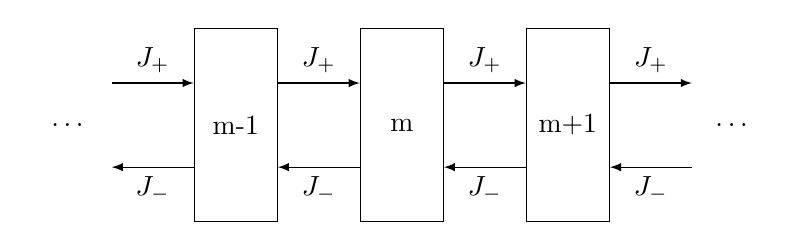
\begin{tikzpicture}[>=latex]
        %[set style={{help lines}+=[dashed]}, scale=0.85, 
        %every node/.style={scale=1}]
        \tikzstyle{state} = [draw, fill=white, rectangle, 
            minimum height=7em, minimum width=3em, node distance=6em]
        \tikzstyle{state2} = [draw=white, fill=white, rectangle, 
            minimum height=7em, minimum width=3em, node distance=6em]
        \tikzstyle{stateEdgePortion} = [black];
        \tikzstyle{stateEdge} = [stateEdgePortion,->];
        \tikzstyle{edgeLabel} = [above, pos=0.5, text centered];
        \tikzstyle{edgeLabel2} = [below, pos=0.5, text centered];
        \node[state] (nodeM) {m-1};
        \node[state, right of=nodeM] (nodeN) {m};
        \node[state, right of=nodeN] (nodeO) {m+1};
        \node[state2, left of=nodeM] (nodeL) {\ldots};
        \node[state2, right of=nodeO] (nodeP) {\ldots};

        \draw (nodeM.45)
        edge[stateEdge] node[edgeLabel]{$J_+$} 
        (nodeN.135);
        \draw (nodeN.45)
        edge[stateEdge] node[edgeLabel]{$J_+$} 
        (nodeO.135);
        \draw (nodeO.45)
        edge[stateEdge] node[edgeLabel]{$J_+$} 
        (nodeP.135);
        \draw (nodeL.45)
        edge[stateEdge] node[edgeLabel]{$J_+$} 
        (nodeM.135);
        
        \draw (nodeN.225)
        edge[stateEdge] node[edgeLabel2]{$J_-$} 
        (nodeM.315);
        \draw (nodeP.225)
        edge[stateEdge] node[edgeLabel2]{$J_-$} 
        (nodeO.315);
        \draw (nodeO.225)
        edge[stateEdge] node[edgeLabel2]{$J_-$} 
        (nodeN.315);
        \draw (nodeM.225)
        edge[stateEdge] node[edgeLabel2]{$J_-$} 
        (nodeL.315);
    \end{tikzpicture}
    \caption{Example of 1-D ERMM node connections.  The outgoing conditions 
$J$ for 
a given node are the incident conditions on the adjacent node.  Each node is 
computed individually, and the global solution is found by sweeping across all 
nodes.}
    \label{fig:ERMM_nodes}
\end{figure*}

In this case, the outgoing information is a boundary flux or current.  
The key 
to response matrix methods is that the outgoing conditions of a cell are 
not passed completely, but rather are projected onto a finite, orthogonal 
basis, and the coefficients of the resulting expansion become unknowns for the 
problem space.  This projection reduces the number of degrees of freedom and, 
thus, reduces the size of the problem. An expansion is completed for each 
phase-space variable (i.e., space, angle, and energy), and the success of these 
expansions depends primarily on the selection of appropriate orthogonal bases 
for each phase-space variable. Response matrix methods  are expensive in 
general,
unless the problem space is greatly reduced in terms of the degrees of 
freedom as compared to more direct solutions.  Thus, proper basis selection is 
paramount if ERMM is to compare in speed and accuracy to other methods for 
solving the transport equation.

In short, basis sets that capture the detail of a high-fidelity transport 
solution with low-order expansions are ideal for ERMM because fewer 
degrees of freedom are needed to achieve the desired accuracy, which reduces 
the problem space, and leads to an easier problem to solve computationally. 
This 
work builds on the previous effort presented by \citet{RobertsSerment}, which 
explored spatial and angular expansions in ERMM.  This work extends their 
progress by utilizing a new, highly successful energy basis for use in ERMM 
based on the Karhunen-Lo\`{e}ve transform, which is discussed in detail in 
\CHAPTER{Chapter3}.  These basis sets are applied to several illustrative 
problems, which provide insight to the success of the method. 

It is possible (and typical) to use different basis expansions for each 
variable; thus the expansion for each variable can be studied mostly 
independently of the other variables.  However, there exists coupling between 
each phase-space variable. For example, the error caused by the expansion in 
energy is influenced by the expansion in space. This work used reference 
cases 
designed to isolate the effect of only one variable to the best extent 
possible. 
 These reference cases are described in \CHAPTER{Chapter4}.

%-------------------------------------------------------------------------------


\subsection{Mathematical Formulation of ERMM}

The following is a presentation of the time-independent, eigenvalue response 
matrix method.  Although the following method is most closely 
linked to the work of \citet{RobertsSerment}, a presentation akin to 
that of \citet{roberts2014hot} has been adapted for this work.  For 
time-independent, multigroup problems, \EQ{eq:fundamentaleq} may be rewritten as
\begin{equation}
    \begin{split}
        \oper{T}\psi^{\mathrm{global}}(\vec{r},\vec{\Omega},g) = 
        \frac{1}{k} \oper{F} \psi^{\mathrm{global}}(\vec{r},\vec{\Omega},g)  
        \, ,
    \end{split}   
    \label{eq:global}
\end{equation}
where $\rho$ has been replaced by the spatial coordinate $\vec{r}$, the 
direction of travel $\vec{\Omega}$, and the energy group $g$. 

The ``global'' superscript in \EQ{eq:global} indicates that the equation defines 
balance for the full problem of interest, and thus is the complete or global 
solution.  ERMM works by breaking the global problem into small, independent or 
local nodes. To do so, let the global volume $V$ be decomposed into $I$ 
disjoint, convex, nodal 
sub-volumes $V_i$ that satisfy $V = V_1 \bigcup V_2 \bigcup \cdots \bigcup 
V_I$. Furthermore, let the surface $\partial V_i$ of $V_i$ be composed of
$S$ disjoint, planar surfaces $\partial V_{is}$ that satisfy $\partial V_i = 
\partial V_{i1} \bigcup \cdots \bigcup \partial V_{iS}$. While unnecessary, 
the condition of planar surfaces permits a compact notation.  Finally, let 
$\vec{r}_i$ and $\vec{r}_{is}$ be shorthand for the variable $\vec{r}$ 
confined to values $\vec{r}\in V_i$ and $\vec{r} \in \partial V_{is}$, 
respectively. 

Thus, the equivalent ``local'' transport equation for the $i$th node is
\begin{equation}
    \oper{T}\psi^{\mathrm{local}}(\vec{r}_i,\vec{\Omega},g) = 
    \frac{1}{k} \oper{F} \psi^{\mathrm{local}}(\vec{r}_i,\vec{\Omega},g) \, ,
    \label{eq:local}
\end{equation}
subject to  $S$  incident-flux boundary conditions 
\begin{equation}
    \psi^{\mathrm{local}}(\vec{r}_{is}, \vec{\Omega}, g) = 
    \psi^{\mathrm{global}}(\vec{r}_{is},\vec{\Omega}, g) \, ,
    \quad \vec{\Omega} \dotp \vec{n}_{is} < 0 \, ,
    \label{eq:localbc}
\end{equation}  
where the unit vector $\vec{n}_{is}$ is the outward normal of surface 
$\partial V_{is}$. \EQUATIONSTWO{eq:local}{eq:localbc} can be combined by 
casting 
incident-flux conditions as external sources such as, 
\begin{equation}
    \left ( \oper{T} - \frac{1}{k} \oper{F} \right 
    )\psi^{\mathrm{local}}(\vec{r}_i,\vec{\Omega},g) = 
    j^{\mathrm{global}}(\vec{r}_i, \vec{\Omega},g) 
    \delta(\vec{r}_i \dotp \vec{n}_{is}) \, ,  
    \label{eq:localcombined}
\end{equation}
where $\vec{j} = \vec{\Omega} \psi$ is the angular current vector, and $j$ is 
the magnitude of the angular current.  For brevity, $j$ is referred to as the 
angular current. This 
formulation allows the global problem to be formed by sweeping across each 
local node.

The general solution of \EQ{eq:localcombined} for arbitrary incident conditions 
can be expressed as the convolution of the external source term with an 
appropriate kernel, or
\begin{equation}
    \begin{split}
        \psi(\vec{r}_i, \vec{\Omega},g) =   
        \sum^{G}_{g'=1} &  \sum^{S}_{s'=1}  
        \int\limits_{\vec{n}_{is'} \dotp \vec{\Omega}' < 0} 
        %\times \\ & 
        R_{f}(\vec{r}'_{is'},\vec{\Omega}',g' \to 
        \vec{r}_i,\vec{\Omega},g)        
        j (\vec{r}'_{is'},\vec{\Omega}', g') \, d\Omega \, ,             
    \end{split}           
    \label{eq:localflux}
\end{equation}
where $G$ is the number of groups, and the ``local'' and ``global'' superscripts 
have been omitted. Similarly, exiting angular currents can be expressed as 
\begin{equation}
    \begin{split}
        j^+(\vec{r}_{is},\vec{\Omega},g) &= \\
        \sum^{G}_{g'=1} &  \sum^{S}_{s'=1}  \,
        \int\limits_{\vec{n}_{is'} \dotp \vec{\Omega}' < 0} 
        %\times \\ &
        R_{c}(\vec{r}'_{is'},\vec{\Omega}' ,g' \to 
        \vec{r}_{is},\vec{\Omega},g)        
        j (\vec{r}'_{is'},\vec{\Omega}', g') \, d\Omega \, , 
    \end{split}   
    \label{eq:localj}
\end{equation}
where $\vec{n}_{is} \dotp \vec{\Omega} > 0$. The integration kernels $R_{f}$ 
and 
$R_{c}$ are $f$lux- and $c$urrent-response functions, which represent 
the angular flux and outgoing angular current at one point in phase-space due 
to a unit, incident current at another point in phase-space.  However, some 
effort is required to convert 
\EQSTWO{eq:localflux}{eq:localj} into a practical form.  The goal is 
to 
reduce the effort needed to compute the global solution; thus, some 
approximations should be made for each phase-space variable.

\subsection{Projection onto a Space and Angle Subspace}

The first approximations are the treatment of the angular and spatial 
dependence.  Projection of local angular currents and fluxes onto a finite 
subspace represented by an orthogonal basis allows the use of a truncated 
basis to represent space and angle.  Using a truncated basis reduces the 
problem space, and, hence, the computation cost of ERMM at the expense of 
reduced accuracy. 
Let a finite basis be constructed with a set of functions 
$P^m(\vec{r},\vec{\Omega})$, $m=0,\, 1,\, \ldots \, M$, that are orthonormal 
over some domain of interest (i.e., a volume or a surface).  Then the angular 
flux can be approximated as
\begin{equation}
    \psi(\vec{r}_i, \vec{\Omega}, g) 
    \approx \sum^M_{m=0} \psi_{i}^m(g) P^m_f(\vec{r}_i,\vec{\Omega}) \, ,
    \label{eq:qexpand}   
\end{equation}
where 
\begin{equation}
    \psi_{i}^m(g) = \int_{V_i} \int_{4\pi}
    \psi(\vec{r}_i, \vec{\Omega}, g)  P^m_f(\vec{r}_i,\vec{\Omega})
    \, d\Omega d^3 r_i 
\, ,
\end{equation}
and the $f$ subscript denotes a basis suitable for the angular flux.  Angular 
currents can similarly be approximated as 
\begin{equation}
    j^{\pm}(\vec{r}_{is}, \vec{\Omega}, g) 
    \approx \sum^L_{l=0} j_{is}^{\pm l}(g) 
    P^l_c(\vec{r}_{is},\vec{\Omega}) \, , 
    \quad \vec{n}_{is} \dotp \vec{\Omega} \gtrless 0 \, ,
    \label{eq:jexpand}   
\end{equation}
where 
\begin{equation}
    j_{is}^{\pm l}(g)
    =  \int_{\partial V_{is}} 
    \int\limits_{\vec{n}_{is} \dotp \vec{\Omega} \gtrless 0} 
    j(\vec{r}_{is}, \vec{\Omega},g)  P^l_c(\vec{r}_{is},\vec{\Omega})
    \, d\Omega d^2 r_{is}\, ,
\end{equation}
and the $c$ subscript denotes a basis suitable for the angular current defined 
on a boundary surface.  Then, substitution of \EQSTWO{eq:qexpand}{eq:jexpand} 
into \EQ{eq:localflux}  yields
\begin{equation}
    \begin{split}
        \sum^M_{m=0} \psi_{i}^m(g) P^m_f(\vec{r}_i,\vec{\Omega}) \approx  
        \sum^{G}_{g'=1}  \sum^{S}_{s'=1} \sum_{l'=0}^L  j^{-l'}_{is'}(g') 
        \braket{ R_{f}, P^{l'}_c }    \, ,             
    \end{split}           
    \label{eq:localfluxexpand}
\end{equation}
where variables have been suppressed and $\braket{\cdot}$ indicates the 
appropriate space and angle integration.  Multiplication of 
\EQ{eq:localfluxexpand} by $P^{m}_{f}(\vec{r}_i, \vec{\Omega})$ and
integration of the result over space and angle leads to a set of flux moments 
defined by
\begin{equation}
    \begin{split}
        \psi^{m}_{i}(g) \approx 
        \sum^{G}_{g'=1} \sum^{S}_{s'=1} \sum_{l'=0}^L  
        j^{-l'}_{is'}(g') R^{s'l' \to m}_{fi}(g'\to g)  \, ,
    \end{split}           
    \label{eq:fluxmoments}
\end{equation}
where
\begin{equation}
    R^{s'l' \to m}_{fi}(g'\to g) \equiv  
    \braket{ \braket{ R_{f}, P^{l'}_f}, P^{m}_f} \, .
\end{equation}
Similarly, the outgoing angular currents can also be projected to yield the 
moments
\begin{equation}
    \begin{split}
        j^{+l}_{is}(g) \approx 
        \sum^{G}_{g'=1} \sum^{S}_{s'=1} \sum_{l'=0}^L  
        j^{-l'}_{is'}(g') R^{s'l' \to sl}_{ci}(g'\to g)  \, .        
    \end{split}              
    \label{eq:jmoments}
\end{equation}

By choosing appropriate basis sets for expanding the spatial and angular 
variables, few terms are required for sufficient accuracy.  For this work, 
Jacobi 
polynomials were used for the angular expansion, and Discrete Legendre 
Polynomials were used for the spatial expansion.  The work did not focus on 
optimization of the spatial and angular basis functions, but rather the best 
cases from the work of \citet{RobertsSerment} were used.

\subsection{Projection onto an Energy Group Subspace}

This work focused on the basis sets for energy expansion, and the 
projection for energy is formulated similarly to the space-angle 
projection.  This treatment will eliminate an explicit dependence on $g$. 
Because $g$ is a discrete variable, bases used to represent 
dependence on $g$ consist of discrete functions $P^h(g), \, h = 0,\, 1,\, 
\ldots, \, H$ that satisfy 
\begin{equation}
    \sum^G_{g} P^h(g) P^{h'}(g) = \delta_{hh'} \, ,
\end{equation}
where $\delta_{hh'}$ is the Kronecker-$\delta$.  By using such a discrete 
basis, group-dependent flux moments defined by \EQ{eq:fluxmoments} can be 
approximated as
\begin{equation}
    \psi^{m}_{i}(g) \approx \sum_{h=0}^H  \psi^{mh}_{i} P^h(g) \, ,
    \label{eq:groupfluxmoments}
\end{equation}
where 
\begin{equation}
    \psi^{mh}_{i} = \sum^G_{g=1}   \psi^{m}_{i}(g) P^h(g) \, .
    \label{eq:groupcoefficients}
\end{equation}
Likewise, current moments defined by \EQ{eq:jmoments} can be approximated as
\begin{equation}
    j^{l}_{is}(g) \approx \sum_{h=0}^H  j^{lh}_{is} P^h(g) \, ,
    \label{eq:groupcurrentmoments}
\end{equation}
where 
\begin{equation}
    j^{lh}_{is} = \sum^G_{g=1}   j^{l}_{i}(g) P^h(g) \, .
    \label{eq:groupcurrentcoefficients}
\end{equation}
Substitution of \EQSTWO{eq:groupfluxmoments}{eq:groupcurrentmoments} into 
\EQ{eq:fluxmoments} yields

\begin{equation}
        \sum_{h=0}^H  \psi^{mh}_{i} P^h(g) \approx 
        \sum^{G}_{g'=1} \sum^{S}_{s'=1} \sum_{l'=0}^L \sum^{H}_{h'=0}
        j^{-l'h'}_{is'}(g') 
         \braket{ \braket{ R_{f}, P^{l'}_f}, P^{m}_f} \, .
\end{equation}
Next, multiplication of the result by $P^h(g)$, and summation over energy 
leads to
\begin{equation}
    \psi^{mh}_{i} \approx 
    \sum^{S}_{s'=1} \sum_{l'=0}^L \sum^{H}_{h'=0} 
    j^{-l'h'}_{is'}  R^{s'l'h' \to mh}_{fi} \, ,
    \label{eq:finalfluxmoments}
\end{equation}
where
\begin{equation}
    R^{s'l'h' \to mh}_{fi} \equiv  
    \braket{ \braket{ \braket{ R_{f}, P^{l'}_f}, P^{m}_f}, P^{h}} \, ,
\end{equation}
and the outer brackets represent summation, not integration over $g$. Similarly, 
current moments are defined as
\begin{equation}
    j^{+lh}_{is} \approx 
    \sum^{S}_{s'=1}  \sum_{l'=0}^L \sum^{H}_{h'=0} 
    j^{-l'h'}_{is'}  R^{s'l'h' \to slh}_{ci} \, ,
    \label{eq:finalcurrentmoments}
\end{equation}
where
\begin{equation}
    R^{s'l'h' \to slh}_{ci} \equiv  
    \braket{ \braket{ \braket{ R_{c}, P^{l'}_c}, P^{l}_c}, P^{h}} \, .
\end{equation}

Computation of response function moments $R^{s'l'h' \to mh}_{fi}$ and $R^{s'l'h' 
    \to slh}_{ci}$ requires evaluation of \EQSTWO{eq:localflux}{eq:localj} in 
which the incident current is equal to $P^{l'}_c(\vec{r}_{is'}, \vec{\Omega}) 
P^{h'}(g)$ for each 
allowed combination of $i$, $s$, $l$, and $h$.

\subsection{Response Matrix Formalism}

\EQUATIONSTWO{eq:finalfluxmoments}{eq:finalcurrentmoments} can be represented as 
nodal response matrix equations, i.e.,
\begin{equation}
    \begin{split}
        \vec{\psi}_i    &=  \mathbf{R}_{fi}  \vec{j}^-_i  \\ 
        \vec{j}^+_i &=  \mathbf{R}_{ci} \vec{j}^-_i  \, ,
    \end{split}
\end{equation}
where  $\vec{\psi}_i$ and $\vec{j}^{\pm}_i$ are vectors of nodal moments and 
$\mathbf{R}_i$'s are matrices of nodal response function moments. Response 
matrix equations for the entire spatial domain can then be written as
\begin{equation}
    \begin{split}
        \vec{\psi}    &= \mathbf{R}_{f} \vec{j}^-  \\
        \vec{j}^+ &= \mathbf{R}_{c}  \vec{j}^- \, .
    \end{split}
\end{equation}
By redirecting outgoing currents from one node as incident currents to another 
via $\vec{j}^- = \mathbf{Mj}^+$, where the matrix $\mathbf{M}$ represents 
geometry and boundary conditions, the global equations become
\begin{equation}
    \begin{split}
        \vec{\psi}    &= \mathbf{R}_{f}  \vec{j}^-  \\
        \vec{j}^- &= \mathbf{MR}_{c}   \vec{j}^- \, .
        \label{eq:globalrme}
    \end{split}
\end{equation}

In this formulation, the flux is dependent only on incident currents, and 
the response matrices $\mathbf{R}_{f}$ and $\mathbf{R}_{c}$ are functions of 
the $k$-eigenvalue.  When $k$ is not converged, the balance defined by 
\EQ{eq:globalrme} generally does not have a solution. As an alternative, the 
current equation can be rewritten as the nonlinear eigenvalue equation
\begin{equation}
    \mathbf{MR}_{c}(k)   \vec{j}^- = \lambda \vec{j}^- \, .
    \label{eq:lambdaeig}
\end{equation}
After determining $\vec{j}^-$ by solving \EQ{eq:lambdaeig} 
for an assumed value of $k$, the flux and other volume moments can be 
determined.  
Subsequently, a 
new value for $k$ is generated similarly to the traditional power method by 
using the standard balance relation of gains-to-losses.  The new $k$ is then 
used to find $\vec{j}^-$, etc., until the solution has converged. A more 
detailed presentation of algorithms for solving the response matrix equations 
is given by \citet{RobertsSerment}.

%-------------------------------------------------------------------------------

\section{Objectives}

The primary focus of this work is to reduce by an order of magnitude the number of 
energy degrees of freedom needed to achieve sub-$0.1\%$ 
error or better in the relative fission density error or pin powers. The 
fission density is 
directly related to the power levels throughout the problem.  To evaluate the method, 
several test problems were devised to test the energy expansion including two 
1-D problems and one 2-D problem.  The project tested several facets of the 
orthogonal basis sets produced by the Karhunen-Lo\`{e}ve Transform (KLT), which 
was used for expansion in energy.  

The KLT uses snapshots (discussed in detail in \CHAPTER{Chapter4}) to 
generate the basis sets.  Thus, the work has considered several different 
models from which to generate snapshots.  Each unique set of basis functions is 
used to expand the energy dependence for the test problem, and results are 
generated as 
the relative error in the fission density for the expansion as a function of 
order.  The results of the 1-D test problems are presented in 
\CHAPTER{Chapter5}, while the results of the 2-D test problem are presented 
in 
\CHAPTER{Chapter6}.  During the course of the project, several parametric 
studies were developed to test the impact of different aspects of the models.  
These parametric studies are presented in Appendix \ref{AppendixA}.